\chapter{Modelling the grid}
\label{chp:Modeling_the_grid}
\section{Voltage-converters in grids}
\label{sec:VSC}


\begin{figure}[ht!]
 \centering
 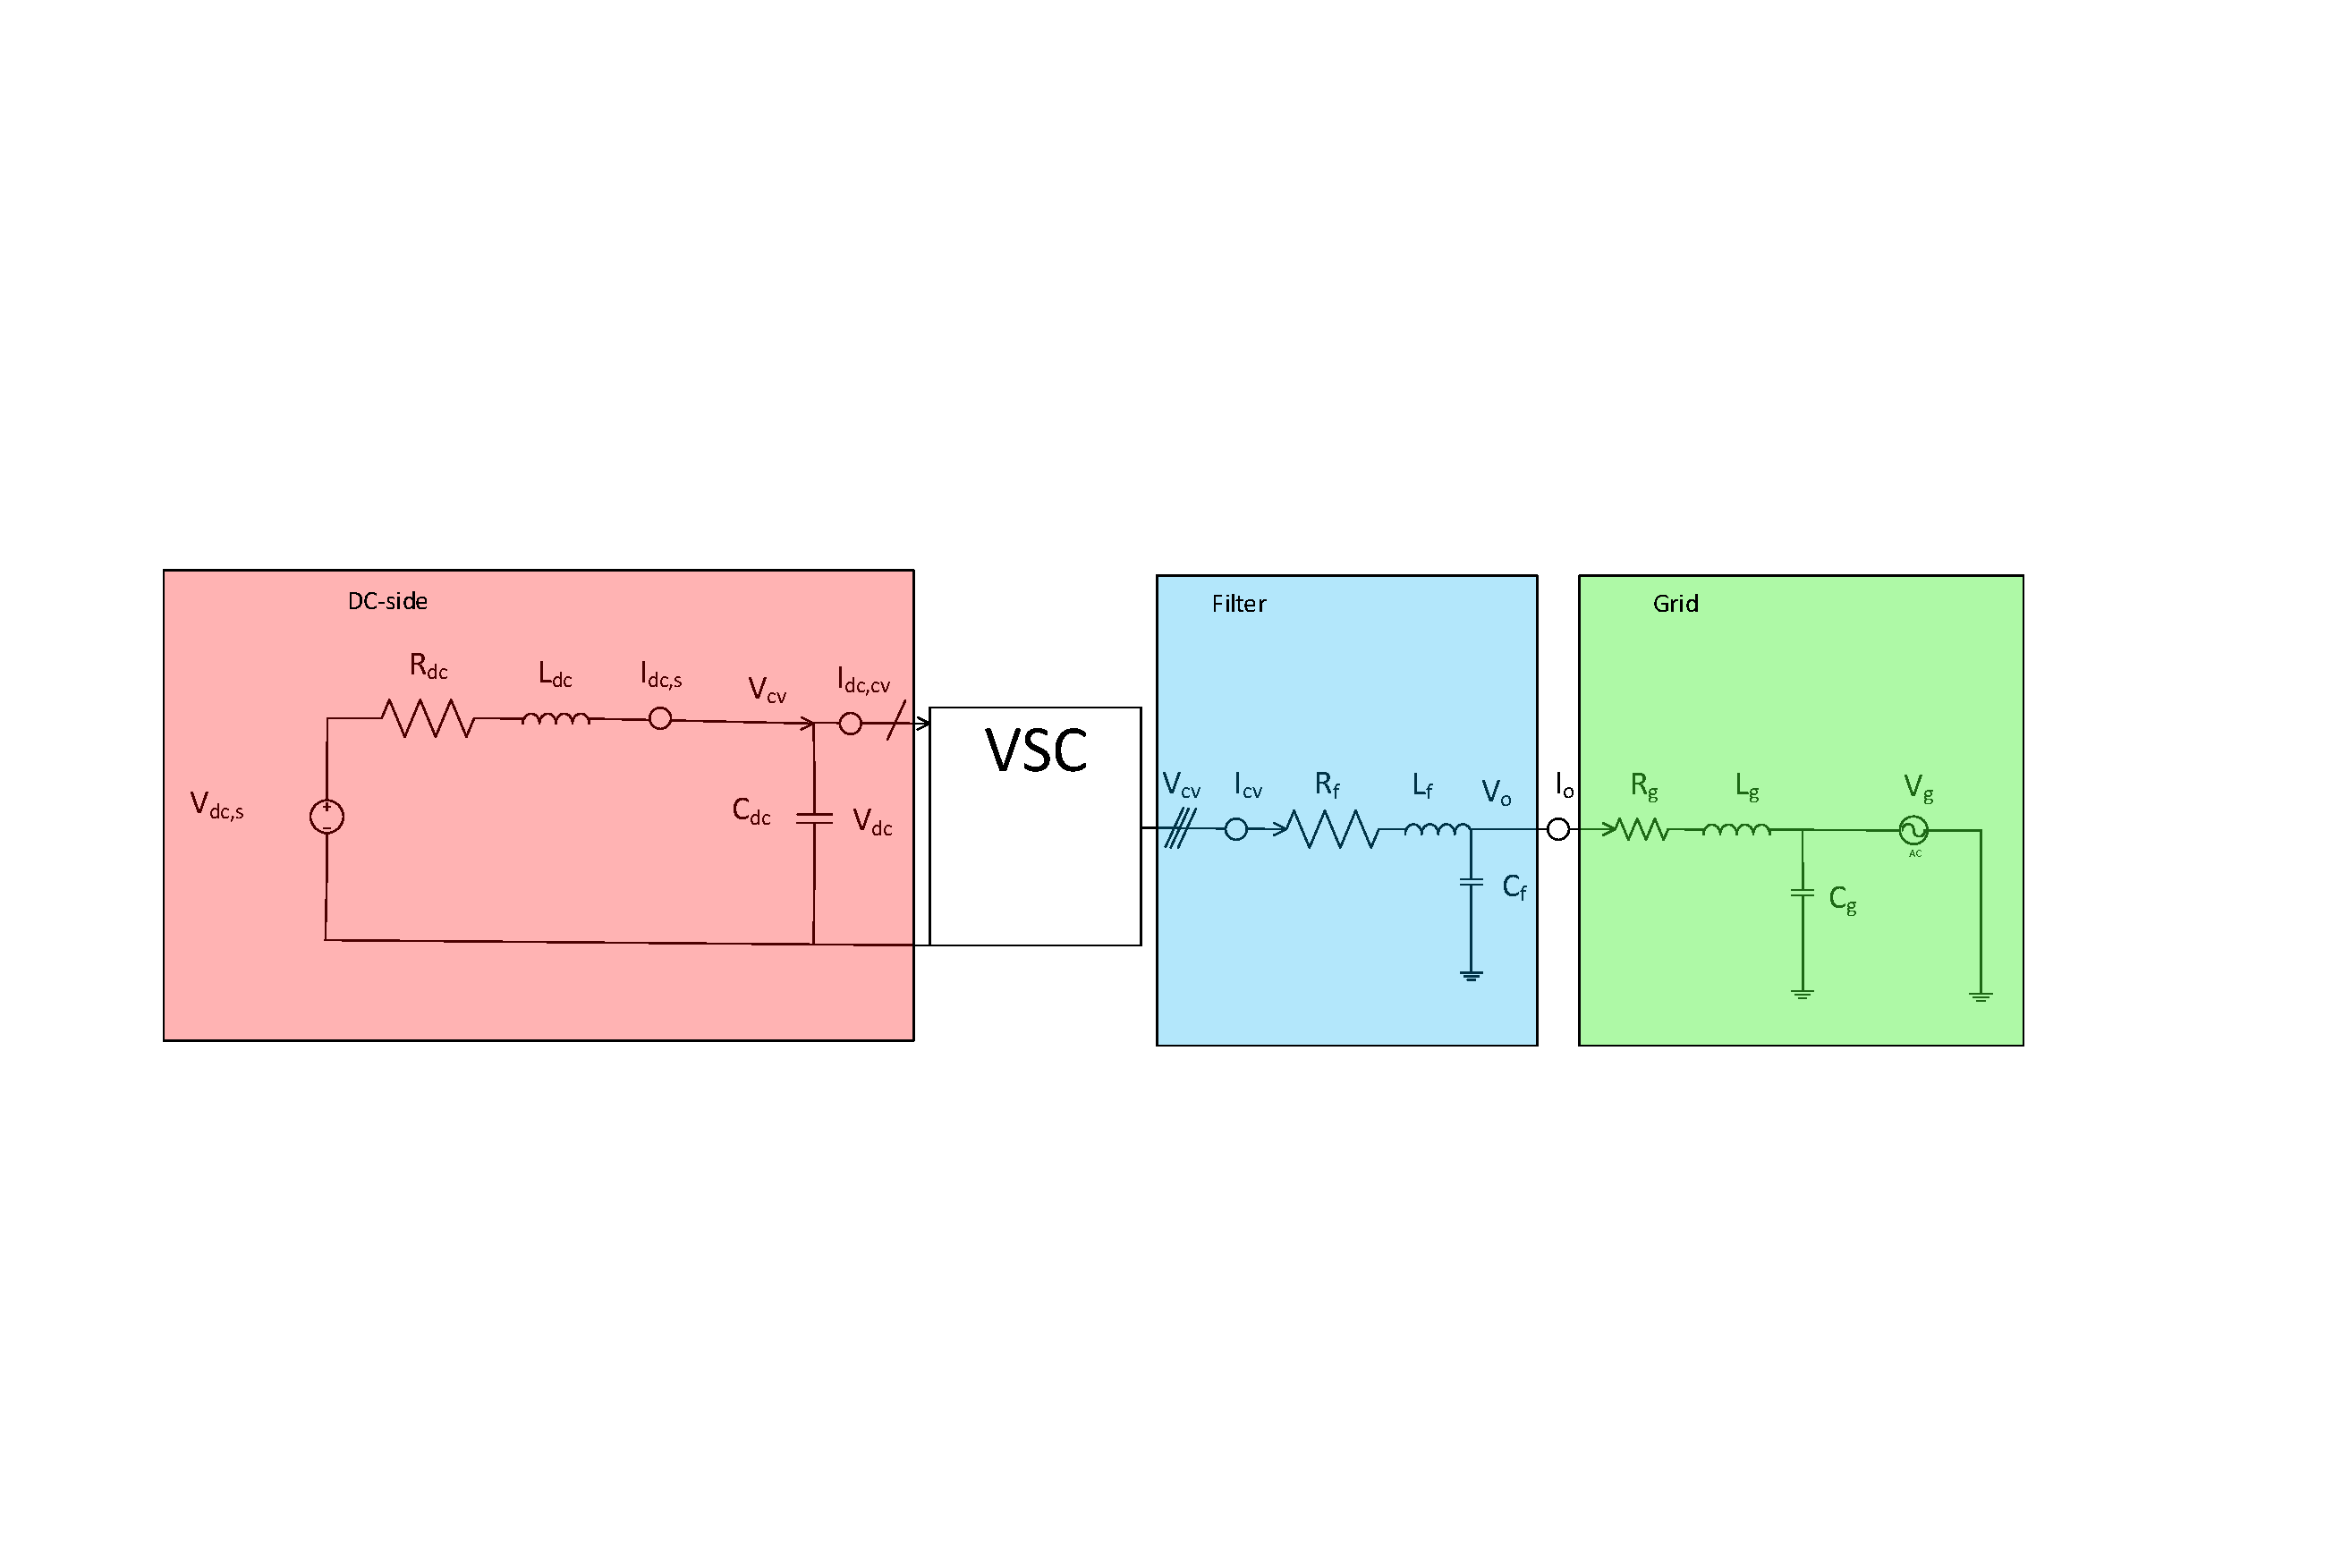
\includegraphics[width=\textwidth,height=\textheight,keepaspectratio]{Figures/Sectioned_simplest_transformer.pdf}
 \caption{The circuit with the VSC as a black box. The components are divided into sections for clarity}
 \label{fig:simplest_system}
\end{figure}


In order to connect a DC-voltage source to an AC power-grid, some kind of transformation is needed. Usually, this is done with a \gls{VSC}, as sin in \cref{fig:simplest_system}. We will represent the internal impedance by the components R\gls{_dc}, L\gls{_dc} and C\gls{_dc} on the dc-side side of the \gls{VSC}. In order to create a smooth current and voltage from the voltage \gls{V_cv}, and the current \gls{I_cv}, a first-order continuous filter is made. The filter is made up of R\gls{_f},L\gls{_f} and C\gls{_f}. For simplicity, the output of the \gls{PWM} is assumed to be a piecewise constant signal, even though it, in reality, is a duty-cycle. The grid can be modeled in a lot of different ways, depending on if there are other components, or if it is a strong grid. The simplest possible model is with a strong grid, which means the voltage of the grid is an AC-voltage that does not change depending on the current given or taken to the grid. 

As seen in \cite{Suul_paper_1}, the internal impedance and the line-impedance on the DC-side can be modeled as a pi-equivalent ( an inductor and a resistor in series, followed by a capacitor in parallel). Also, any capacitance at the terminal is simply added as a part of the inductor. The line-impedances along in the AC-grid can also be lumped together into a pi-equivalent, just like in \cite{Suul_paper_1}
\noindent
%#TODO Legg finn ut hvor jeg skal skrive om VSC-en
If a \gls{PWM} is supposed to be able to follow the voltage from somewhere else, it needs to know the phase and frequency of the rest of the grid. Since none of these are known exactly, some kind of measurement is needed to provide them instead. This is where the \gls{PLL} comes in. The \gls{PLL} is a part of the \gls{VSC}. It takes the measured voltage at the output of the filter and is give an output that converges towards the actual angle and angular velocity of the grid. The \gls{PLL} is discussed further in \cref{sec:PLL}


\begin{figure}[ht!]
 \centering
 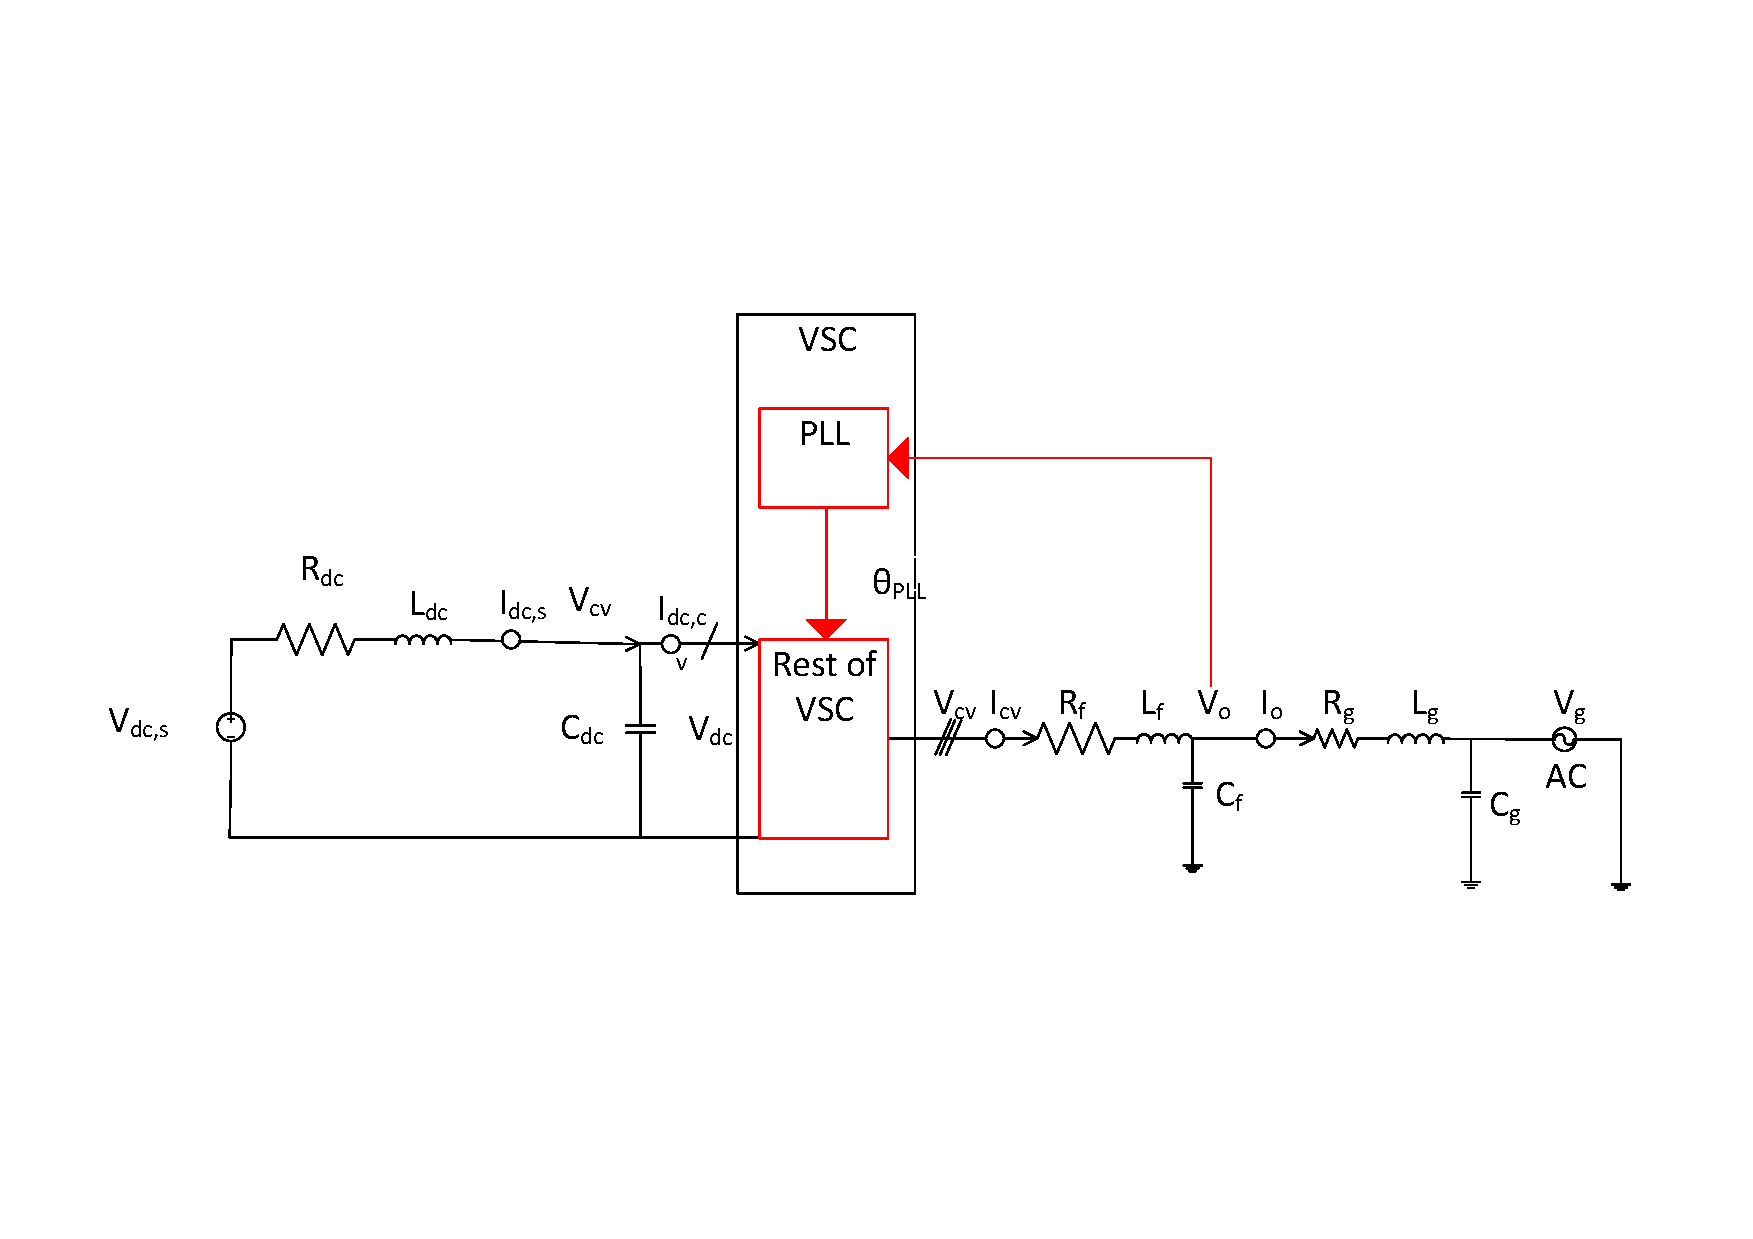
\includegraphics[width=\textwidth,height=\textheight,keepaspectratio]{Figures/Transformer_with_PLL.pdf} %#TODO Make a better figure that adds the PLL to the VSC
 \caption{The \gls{PLL} is a part of the \gls{VSC} that gives an estimate of the phase, which is reeded for the rest of the \gls{PLL} to function. It will be discussed properly in \Cref{sec:PLL}}
 \label{fig:curcuit_with_pll}
\end{figure}

A normal PI-controller will not be able to follow an oscillating reference that has an unknown frequency without suffering from stationary deviations. The solution for this is to use a rotating reference frame. 


\section{The Park transformation}

A proper explanation of the dqz- transformation is in \cref{sec:rotating_reference_frame}

The dqz-transformation can be seen as a projection from the normal reference-frame, abc, to a rotating reference-frame, dq. An alternating current that has the same angular velocity as the dq-reference frame will be perceived as a complex, stationary DC-current instead in the dq-frame. For a balanced system, the transformation is given by the matrix

\begin{equation}
 K_{CP} = 
 \frac{2}{3}\begin{bmatrix}
 \cos{\left(\theta\right)}
 & \cos{\left(\theta - \frac{2\pi}{3}\right)}
 & \cos{\left(\theta + \frac{2\pi}{3}\right)} \\
 -\sin{\left(\theta\right)}
 & -\sin{\left(\theta - \frac{2\pi}{3}\right)}
 & -\sin{\left(\theta + \frac{2\pi}{3}\right)} 
\end{bmatrix}
\end{equation}{}

The third state is a scaled sum of all phases, but since all phases are supposed to add up to 0 together in a balanced system, they are ignored here. 

\noindent
The transformation makes it possible to view the control problem as time-invariant. This is because the reference signal from the grid-voltage will no longer have to be viewed as three oscillating sine-waves, but instead as two signals that will remain constant as long as the grid-voltages continue to oscillate with the same amplitude and frequency. This is especially useful since linear regulators have no way to follow an arbitrary single frequency without phase-delay.

\section{Per unit systems}
Normally, an electrical system is designed with regard to some specific physical parameters. This means that using the same design for systems with different characteristics requires some thought when scaling all the parameters. 
Per-unit systems help to solve this by defining nominal values (The normal values of both components and states during "Normal operation"), and then designing the circuit with values that are expressed as multiples of the base-values instead. This makes it easier to use the same design for several different scenarios. It also makes it easier to see if observed values are abnormal or not, since everything is based around 1. Basis values for a per-unit system are always followed by a subscript b (like V\gls{_b}). A value that is given in per unit will always be written as a lowercase letter. Physical values, except for angular velocity $\omega$ are always written in upper-case. 


\begin{equation}
 v_g = \frac{V_g}{V_b}
\end{equation}{}

In order to get a per-unit system, some base values have to be defined. These are usually $P_b$, $\omega_b$ and $V_b$. Take note that $\omega_b$ breaks the convention since all angular velocities are all given by a small $\omega$, regardless if they are per unit or not. The grid frequency \gls{omega_g}, estimated grid frequency $\omega_{PLL}$ and basis frequency $\omega_b$ are all written in lower-case, even though only the first two are in per unit. We do this because large $\Omega$ usually refers to a resistance of some sort. As a result: 
\begin{equation}
 \gls{omega_g} = \frac{\omega_{g, physical}}{\omega_{b}} 
\end{equation}
\section{Circuit equations}
As seen in \cite{Suul_paper_1}, the internal impedance and the line-impedance on the DC-side can be modeled as a pi-equivalent (An inductor and a resistor in series, followed by a capacitor in parallel). Also, any capacitance at the terminal on the DC-side described within the capacitance in the pi-equivalent. The filter is a simple RLC-filter, just like what can be seen in \cref{fig:simplest_system}.

In order to get the circuit equations for the dq-reference frame, some assumptions and observations have to be made. 
Firstly, the $\alpha\beta$-frame is just a constant linear combination of the abc-frame. This means that, due to linearity, the differentiating variables in the $\alpha\beta$-frame will act exactly like the ones in the $abc$-frame. 
Also, anything in the dq-frame can be represented as $v_{dq} = e^{-j\theta_{PLL}} v_{\alpha\beta}$. As long as the angular velocity remains constant, it can be written as $v_{dq} = e^{-j\left(\omega_{PLL} t + \phi \right)} v_{\alpha\beta}$. This means that 
\begin{equation}
 \frac{d \left( i_{dq} \cdot e^{\omega_b t}\right) }{dt} = e^{\omega_b t} \left( \omega_b i_{dq} + \frac{d i_{dq}}{dt} \right) 
\end{equation}
As a result, differentiation in the dq-frame acts differently than in the $\alpha\beta$-frame, but can still be done. 
Finally, the fact that $I_b R_b = I_b \omega_b L_b$ in the dq-frame is also used to get the normal circuit-equations on per unit form. As a result the circuit equations can be written as in \cite{Suul_paper_1}: 


\begin{align}
 \frac{d \Vec{i\gls{_cv}}}{dt} &= \frac{\omega\gls{_b}}{l\gls{_f}}\Vec{v_{cv}} - \frac{\omega_b}{l_f}\Vec{v}\gls{_o} - \left( \frac{r_{l_f}\omega_b}{l_f} + j\gls{omega_g}\omega_b \right) \Vec{i_{cv}}\\
 \frac{d \Vec{v\gls{_o}}}{dt} &= \frac{\omega\gls{_b}}{c\gls{_f}}\Vec{i_{cv}} - \frac{\omega_b}{c_f}\Vec{i}\gls{_o} - j\gls{omega_g}\omega_b \Vec{v_{o}}\\
 \frac{d \Vec{i\gls{_o}}}{dt} &= \frac{\omega\gls{_b}}{l\gls{_g}}\Vec{v_{o}} - \frac{\omega_b}{l_g}\Vec{v}\gls{_g} - \left( \frac{r_{g}\omega_b}{l_g} + j\omega_g\omega_b \right) \Vec{i_{o}}\\
\end{align}{}



And on the DC-side, they are:
\begin{align}
 \frac{d v\gls{_dc}}{dt} &= \frac{\omega_b}{c_{dc}}\gls{i_dc,s} - \frac{\omega_b}{c_{dc}}i\gls{_dc}\\
 \frac{d \gls{i_dc,s}}{dt} &= \frac{\omega_b}{l_{dc}}\gls{v_dc,s} - \frac{\omega_b}{l_{dc}}v\gls{_dc}
\end{align}{}